\documentclass[11pt,a4paper]{article}

\usepackage{tikz}
\usetikzlibrary{nfold}
\usetikzlibrary{intersections}
\usetikzlibrary{cd}


\begin{document}

\section{Various tests}

\subsection{Miter limit}

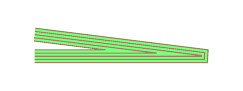
\begin{tikzpicture}[line join=miter, miter limit=16, x={(1.1cm,0)}, y={(0,1.1cm)}]
  \path[draw=green,opacity=0.5, line width=5pt] (0,0) -- (2,0) -- (0,0.25);
  \path[draw=purple, opacity=0.5, double distance=4.2pt, nfold=5] (0,0) -- (2,0) -- (0,0.25);
\end{tikzpicture}
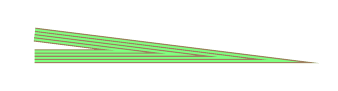
\begin{tikzpicture}[line join=miter, miter limit=17, x={(1.1cm,0)}, y={(0,1.1cm)}]
  \path[draw=green,opacity=0.5, line width=5pt] (0,0) -- (2,0) -- (0,0.25);
  \path[draw=purple, opacity=0.5, double distance=4.2pt, nfold=5] (0,0) -- (2,0) -- (0,0.25);
\end{tikzpicture}

\subsection{Transformed axes with relative and absolute coordinates}

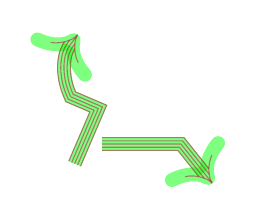
\begin{tikzpicture}[x={(.3cm,.7cm)}, y={(.7cm,-.3cm)}]
  \path[draw=green,opacity=0.5, line width=5pt, arrows=->] (1.5,1.0) -- (2.5,1.0) -- (2.5,0.5)  to[relative, out=30, in=150] (3.5,0.2);
  \path[draw=purple, opacity=0.5, arrows=-Implies, double distance=4.2pt, nfold=5]
      (1.5,1.0) -- (2.5,1.0) -- (2.5,0.5) to[relative, out=30, in=150] (3.5,0.2);
  \path[draw=green,opacity=0.5, line width=5pt, arrows=->] (1.5cm,1.0cm) -- (2.5cm,1.0cm) -- (2.9cm,0.5cm);
  \path[draw=purple, opacity=0.5, arrows=-Implies, double distance=4.2pt, nfold=5] (1.5cm,1.0cm) -- (2.5cm,1.0cm) -- (2.9cm,0.5cm);
\end{tikzpicture}

\subsection{Path with jump and cycle}
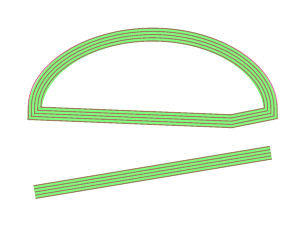
\begin{tikzpicture}
    \path [draw=green,opacity=0.5, line width=5pt] (0,0) -- (3,0.5) (3,1) arc (0:180:1.5 and 1) -- (2.5,0.9) -- cycle;
  \path[draw=purple, opacity=0.5, double distance=4.2pt, nfold=5] (0,0) -- (3,0.5) (3,1) arc (0:180:1.5 and 1) -- (2.5,0.9) -- cycle;
\end{tikzpicture}

\subsection{Different joins in the same diagram}


\begin{tikzpicture}[line join=bevel, double distance=5pt, line width=.5pt, draw=purple, opacity=0.5]
  \path[line join=miter, draw=green, line width=6pt] (0,0) -- (1, 0) -- (0,1);
  \path[draw=green, line width=6pt] (2,0) -- (3, 0) -- (2,1);
  \path[line join=round, draw=green, line width=6pt] (4,0) -- (5, 0) -- (4, 1);
  \path[line join=miter, arrows=|-Implies,  double distance=5pt, nfold=4] (0,0) -- (1, 0) -- (0,1);
  \path[double distance=5pt, nfold=4] (2,0) -- (3, 0) -- (2,1);
  \path[line join=round,  double distance=5pt, nfold=4] (4,0) -- (5, 0) -- (4, 1);
\end{tikzpicture}

\subsection{Shorten}
Shortening needs to be implemented manually, as discussed in the comments.

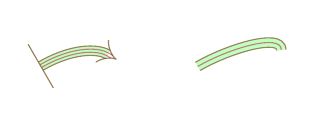
\begin{tikzpicture}
  \draw[draw=green,opacity=.5,double distance=3pt, shorten >= 3pt, shorten <=-2pt, arrows=|-Implies] (0,0) to[bend left] (1,0);
  \draw[draw=purple, opacity=.5,double distance=3pt, shorten >= 3pt, shorten <=-2pt, arrows=|-Implies, nfold=4] (0,0) to[bend left] (1,0);
  \draw[draw=green,opacity=.5,double distance=3pt, shorten >= 5pt, shorten <=-2pt] (2,0) to[out=30,in=90] (3,0);
  \draw[draw=purple, opacity=.5, double distance=3pt, shorten >= 5pt, shorten <=-2pt, nfold=3] (2,0) to[out=30,in=90] (3,0);
\end{tikzpicture}

\subsection{Different types of tips}

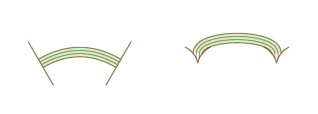
\begin{tikzpicture}
  \draw[draw=green,opacity=.5,double distance=3pt, arrows=|-|] (0,0) to[bend left] (1,0);
  \draw[draw=purple, opacity=.5,double distance=3pt, arrows=|-|, nfold=4] (0,0) to[bend left] (1,0);
  \draw[draw=green,opacity=.5,double distance=3pt, arrows=Implies-Implies] (2,0) to[out=90,in=90] (3,0);
  \draw[draw=purple, opacity=.5, double distance=3pt, nfold=4, arrows=Implies-Implies] (2,0) to[out=90,in=90] (3,0);
\end{tikzpicture}

\subsection{More extreme paths}

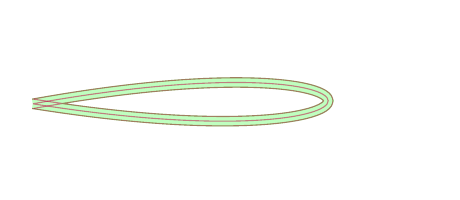
\begin{tikzpicture}
  \draw[draw=green,opacity=.5,double distance=3pt] (0,0) .. controls (5,.9) and (5,-.8) .. (0,0);
  \draw[draw=purple, opacity=.5,double distance=3pt, nfold=3] .. controls (5,.9) and (5,-.8) .. (0,0);
\end{tikzpicture}
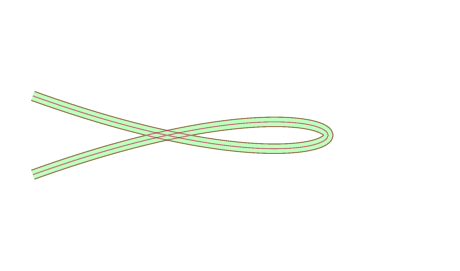
\begin{tikzpicture}
  \draw[draw=green,opacity=.5,double distance=3pt] (0,-.5) .. controls (5, 1.3) and (5,-1.3) .. (0,.5);
  \draw[draw=purple, opacity=.5,double distance=3pt, nfold=3] (0,-.5) .. controls (5, 1.3) and (5,-1.3) .. (0,.5);
\end{tikzpicture}

\subsection{Degenerate paths and tips}
Does not crash, which is good. However, need to consider if this is the desired behaviour.


\begin{tikzpicture}
  \draw[draw=green,opacity=.5,double distance=3pt, arrows=|-|] (0,0) (.25,0) -- (.75,0) (1,0);
  \draw[draw=purple, opacity=.5,double distance=3pt, arrows=|-|, nfold=4] (0,0) (.25,0) -- (.75,0) (1,0);
  \draw[draw=green,opacity=.5,double distance=3pt, arrows=Implies-Implies] (2,0) (2.25,0) -- (2.75,0) (3,0);
  \draw[draw=purple, opacity=.5, double distance=3pt, nfold=4, arrows=Implies-Implies] (2,0) (2.25,0) -- (2.75,0) (3,0);
\end{tikzpicture}


\subsection{Checking for undesired global effects}

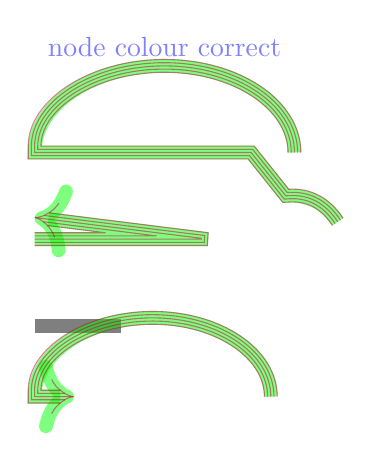
\begin{tikzpicture}[line join=miter, miter limit=10, x={(1.1cm,0)}, y={(0,1.1cm)}]
  \path [draw=green,opacity=0.5, line width=5pt, arrows=->] (3,1) arc (0:180:1.5 and 1) -- (0.5,1.0) -- (2.5,1.0) -- (2.9,0.5)  to[relative, out=30, in=150] (3.5,0.2) (0,0) -- (2,0) -- (0,0.25) ;
  \path[draw=purple, opacity=0.5, arrows=-Implies, double distance=4.2pt, nfold=5]
    (3,1) arc (0:180:1.5 and 1) node[blue, midway, above] {node colour correct} -- (0.5,1.0) -- (2.5,1.0) -- (2.9,0.5) to[relative, out=30, in=150] (3.5,0.2)
  (0,0) -- (2,0) -- (0,0.25);
  % make sure the subsequent path is unaffected
  \draw[line width=5pt, opacity=.5] (0,-1)  -- (1, -1);
    \path[draw=green,opacity=0.5, line width=5pt, arrows=->]
    (3 cm,-2 cm) arc (0:180:1.5 cm and 1 cm) -- (0.5 cm,-2 cm);
    \path
    [draw=purple,decorate,opacity=0.5, arrows=-Implies, double distance=4.2pt, nfold=5]
    (3 cm,-2 cm) arc (0:180:1.5 cm and 1 cm) -- (0.5 cm,-2 cm);
\end{tikzpicture}
%
\section{tikz-cd compatibility}

\begin{tikzcd}[row sep=1.5cm]
      a_2 \ar[d, Rightarrow, double distance=10pt, nfold]
    & a_3 \ar[d, Rightarrow, double distance=10pt, nfold=3]
    & a_4 \ar[d, Rightarrow, double distance=10pt, nfold=4]
    & a_5 \ar[d, Rightarrow, double distance=10pt, nfold=5]
    & a_6 \ar[d, Rightarrow, double distance=10pt, nfold=6]
    & a_7 \ar[d, Rightarrow, double distance=10pt, nfold=7]
    \\
  b_2 \ar[r, Mapsto, nfold] \ar[r, Mapsto, color=green, opacity=.5] & b_3 \ar[r, Mapsto, double distance=3pt, nfold=3] & b_4 \ar[r, Mapsfrom, nfold=3] & b_5 & b_6 & b_7
\end{tikzcd}


\newcommand{\testarrow}[2]{
  \def\testoptions##1{[##1]}
  \expandafter\ar\testoptions{Rightarrow,red,opacity=.8,#1}
  \expandafter\ar\testoptions{Rightarrow,opacity=.7,green!70!black,#1,#2}
}
\begin{tikzcd}[scale=1.1]
  a_1
  \testarrow{dr, shift left=-10pt, shorten <=5pt, shorten >=3pt,
    out=-10, in=110, "l", "m"'}{nfold=3}
  & a_2
  \testarrow{%
    d,double distance between line centers=5pt, "a" inner sep=3.5pt,
    "o"' inner sep=3.5pt, shorten >=-5pt, shorten <=-1pt, bend left=30
  }{nfold=5}
  \\
  b_1 & b_2 \\
  c_1
  \testarrow{d,"a", "b"', bend left=30}{nfold}
  \testarrow{r}{nfold}
  & c_2 
  \testarrow{dr,shift left=-1pt, out=30, in=180,"l", "m"'}{nfold}
  & c_3 \\
  d_1 \testarrow{r, bend right, double distance=5pt, "a","b"'}{nfold=5} & d_2 & d_3
\end{tikzcd}

\end{document}
